%%%%%%%%%%%%%%%%%%%%%%%%%%%%%%%%%%%%%%%%%%%%%%%%%%%%%%%
%% Bachelor's & Master's Thesis Template             %%
%% Copyleft by Artur M. Brodzki & Piotr Woźniak      %%
%% Faculty of Electronics and Information Technology %%
%% Warsaw University of Technology, 2019-2020        %%
%%%%%%%%%%%%%%%%%%%%%%%%%%%%%%%%%%%%%%%%%%%%%%%%%%%%%%%

\documentclass[
    left=2.5cm,         % Sadly, generic margin parameter
    right=2.5cm,        % doesnt't work, as it is
    top=2.5cm,          % superseded by more specific
    bottom=3cm,         % left...bottom parameters.
    bindingoffset=6mm,  % Optional binding offset.
    nohyphenation=false % You may turn off hyphenation, if don't like.
]{eiti/eiti-thesis}

\langpol % Dla języka angielskiego mamy \langeng
\graphicspath{{img/}}             % Katalog z obrazkami.
\addbibresource{bibliografia.bib} % Plik .bib z bibliografią

\begin{document}

%--------------------------------------
% Strona tytułowa
%--------------------------------------
\EngineerThesis % Dla pracy inżynierskiej mamy \EngineerThesis
\instytut{Informatyki}
\kierunek{Informatyka}
\specjalnosc{Inżynieria Systemów Informacyjnych}
\title{
    Generowanie automatycznych podpowiedzi \\w środowiskach do programowania
}
\engtitle{ % Tytuł po angielsku do angielskiego streszczenia
    Generating code autocompletions for Integrated Development Environments 
}
\author{Rafał Lewanczyk}
\album{293140}
\promotor{dr inż. Paweł Zawistowski}
\date{\the\year}
\maketitle

%--------------------------------------
% Streszczenie po polsku
%--------------------------------------
\cleardoublepage % Zaczynamy od nieparzystej strony
\streszczenie \\
Uzupełnianie kodu jest funkcją odpowiedzialną za przewidywanie tego co chce, lub może napisać programista. Poprawnie 
działająca może w znaczący sposób wspomóc oraz uefektywnić jego pracę. Istnieje wiele podejść do tego 
problemu np. przy pomocy metod słownikowych lub parsowania na bieżąco pisanego kodu. 

W tej pracy omawiam podejście polegające na zastosowaniu metod uczenia
maszynowego. Generuje ono posortowaną według prawdopodobieństwa wystąpienia listę sugestii, które mogą zostać wykorzystane 
przez programistę w trakcie pracy nad programem. 

Opisuję badane przeze mnie architektury, oraz porównuję je pod względem skuteczności. Wymieniam 
również napotkane wyzwania. 

Końcowy model został wytrenowany na 9000 plikach w języku Python, pochodzących z publicznie dostępnych 
repozytoriów na serwisie GitHub, oraz oceniony na 4500 plikach. Jego skuteczność wyniosła 
\begin{math}68\%\end{math} dla 5 najlepszych predykcji, a średni czas odpowiedzi 18 ms. 

Model ten został zaimplementowany jako wtyczka do środowiska SublimeText 3. 
\slowakluczowe Uczenie maszynowe, autouzupełnianie, kod źródłowy

%--------------------------------------
% Streszczenie po angielsku
%--------------------------------------
\newpage
\abstract
Code autocompletion is a feature that offers suggestions for what a software developer may want 
to write. Correct suggestions improve efficiency of programmers job. There are a lot of forms 
of code autocompletion, for example using dictionary methods or parsing code online. 

In this paper, I propose approach for code autocompletion using machine learning. It generates 
ranked by its probabilities of occurrences list of suggestions, which can be used by software developer at edit time. 

I describe explored architectures and compare them to each other in order to select the best one. I 
also discuss challenges regarding this approach. 

The final model was trained using 9000 Python source files from publicly available repositories from service
GitHub and evaluated on 4500 files. The evaluation results in \begin{math}68\%\end{math}
accuracy for top 5 suggestions, and mean time of response resulted in 18 ms. 

The system is available as a plugin for integrated development environment SublimeText 3. 
\keywords Machine Learning, Autocomplete, Source Code 

%--------------------------------------
% Oświadczenie o autorstwie
%--------------------------------------
\cleardoublepage  % Zaczynamy od nieparzystej strony
\pagestyle{plain}
\makeauthorship

%--------------------------------------
% Spis treści
%--------------------------------------
\cleardoublepage % Zaczynamy od nieparzystej strony
\tableofcontents

%--------------------------------------
% Rozdziały
%--------------------------------------
\cleardoublepage % Zaczynamy od nieparzystej strony
\pagestyle{headings}

\newpage % Rozdziały zaczynamy od nowej strony.
\section{Praefatio}
\lipsum[1] \cite{goossens93}
\begin{figure}[!h]
	% Znacznik \caption oprócz podpisu służy również do wygenerowania numeru obrazka;
	\caption{Tradycyjne godło Politechniki Warszawskiej}
	% dlatego zawsze pamiętaj używać najpierw \caption, a potem \label
    \label{fig:tradycyjne-logo-pw}
    % Zamiast width można też użyć height, etc. 
    \centering 
\includegraphics[width=0.5\linewidth]{logopw.png}
\end{figure}
\lipsum[2-3]
\begin{figure}[!h]
	\caption{Współczesne logo Politechniki Warszawskiej}
	\label{fig:nowe-logo-pw}
	\centering 
\includegraphics[width=0.5\linewidth]{logopw2.png}
\end{figure}
\lipsum[4-6] Reference to image \ref{fig:nowe-logo-pw}. 
         % Wygodnie jest trzymać każdy rozdział w osobnym pliku.
\newpage % Rozdziały zaczynamy od nowej strony.
\section{Podłoże pracy}
W ciągu ostatnich kilku lat przetwarzanie języka naturalnego bardzo się rozwinęło. Wraz z kolejnymi 
badaniami udało się uzyskać coraz lepsze rezultaty. Jednak dział badający zachowanie tych modeli 
na językach programowania jest nowy, co możemy zaobserwować po zbiorze prac \cite{ml4code}
z nim związanych. Jest w nim dużo miejsca na nowe podejścia oraz badania. W tym rozdziale omówię 
opiszę prace istotne lub podobne do mojej.  


\subsection{Sieci neuronowe w przewidywaniu języków programowania}
Subhasis Das, Chinmayee Shah \cite{contextual_code_completion} porównują ze sobą modele
\begin{itemize}
    \item model z wagami o stałej długości okna (fixed window weight model)
    \item model macierzy wektorów (matrix vector model)
    \item sieć neuronowa z wyprzedzeniem (feed-forward neural network)
    \item model z wyprzedzeniem oraz miękka uwagą (feed-forward model with soft attention)
    \item model rekurencyjny z warstwą GRU
\end{itemize}
Kod wejściowy jest poddany tokenizacji przy pomocy wyrażeń regularnych. Oceniane odbywa się poprzez dokładne
dopasowanie pierwszego przewidzianego tokenu oraz na podstawie 3 najlepszych sugestii. Do treningu oraz testów 
używane są kody bibliotek Django, Twisted oraz jądra systemu Linux. Połowa plików źródłowych jednego z 
projektów używana jest jako zbiór treningowy natomiast druga połowa jako zbiór walidacyjny. Wszystkie modele
osiągają dokładność przewidzeń równą około 80\% dla 3 najlepszych sugestii, najlepiej radzi sobie model miękka uwagą
z dokładnością 83.6\%. Problem słów poza słownikiem rozwiązany jest przy pomocy słownika przypisującego 
token o nieznanej wartości do słowa które wpisał użytkownik. Moja praca różni się tym, że skupiam się 
wyłącznie na sieciach rekurencyjnych, jako że w powyższej warstwa LSTM nie została uwzględniona. Próbuję 
również uogólnić przewidywany kod poprzez trening na znacznie bardziej zróżnicowanych bibliotekach aby sprawić
by wtyczka była użyteczna w bardziej ogólnych zastosowaniach. \\

Hellendoorn i Devanbu przeprowadzili eksperyment polegający na wykonaniu 15000 predykcji dla 
środowiska Visual Studio. Jako zbioru danych używają 14000 plików źródłowych w języku Java. 
W swojej pracy porównują skuteczność modelu n-gram z modelami rekurencyjnymi. 
Prezentują również dynamicznie aktualizowane modele n-gram działające w zagnieżdżonym zasięgu, rozwiązując 
w ten sposób problem skończonego słownika oraz znacznie usprawniając sugestie. Rezultaty tej pracy 
pokazują, że pomimo znacznie lepszych wyników sieci rekurencyjnych w zadaniu modelowania języka 
naturalnego, modele n-gram w niektórych przypadkach radzą sobie lepiej z przewidywaniem kodu. Jednym
z przytoczonych przykładów są metody wbudowane w język, dla których głębokie sieci działają lepiej, 
jednak przegrywają przy często występujących, zróżnicowanych,  mało popularnych bibliotekach zewnętrznych, 
w których model n-gram naturalnie radzi sobie lepiej, jednak przegrywa pod innymi względami. Swoje 
eksperymenty przeprowadzają dla stałych wartości hiperparametrów, w swojej pracy chcę również
zająć się strojeniem wybranych modeli. \\

Pythia \cite{pythia} stworzona przez zespół programistów Microsoftu, w którego skład wchodzą Alexey Svyatkovskiy, Shengyu Fu, Ying Zhao, Neel Sundaresan
jest rozszerzeniem do wtyczki IntelliSense w środowisku Visual Studio Code. W swojej pracy testują zastosowanie najwydajniejszych 
na ten moment modeli sieci rekurencyjnych. Jako zbiór treningowy użyte jest 2700 projektów z serwisu github \cite{github}
które wcześniej zostały poddane rozbiorowi na drzewa składniowe. Model osiąga najlepszą dotychczasową skuteczność wynoszącą
92\% dla najlepszych 5 sugestii oraz bardzo dobry czas odpowiedzi w okolicach 100 ms. Eksperymentu tego nie będę w stanie 
dokładnie odtworzyć ze względu na inne przygotowanie danych wejściowych oraz przez inny zbiór danych (zbiór wykorzystany przez
Pythie nie został udostępniony). Mimo to planuję zaimplementować oraz ocenić wyróżnioną architekturę w moim eksperymencie. 

\subsection {Modele statystyczne w przewidywaniu języków programowania}
Myroslava Romaniuk \cite{pharo} pokazuje, że modele statystyczne, w tym przypadku n-gram, dokładnie 
unigram oraz bigram radzą sobie 
z automatycznym uzupełnianiem kodu. W swojej pracy usprawnia działanie wtyczki do środowiska programistycznego 
Pharo. Zaproponowany model trenuje na 50 projektach w tym języku, osiągając dokładność około 40\%. 
W swojej pracy łącze modele rekurencyjne właśnie z kombinacją modeli unigram oraz bigram.

\subsection {Rozwiązania komercyjne}
W dużej mierze do powstania tej pracy przyczyniły się istniejące już rozwiązania komercyjne. Niestety 
ze względów licencyjnych nie są ujawnione dokładnie mechanizmy stojące za ich działaniem, metody użyte 
do treningu oraz dokładna skuteczność, przez co niemożliwe jest porównanie uzyskanych przeze mnie wyników 
z tymi podejściami. \\

Tabnine \cite{tabnine} jest wtyczką do najpopularniejszych środowisk programistycznych realizującą predykcję kolejnego tokenu w 
większości stosowanych języków programowania. Do jej treningu zostało wykorzystane 2 miliony projektów ze strony github \cite{github}. 
Wtyczka opiera się na GPT-2, które używa architektury transformerów. W jej skład wchodzą również zaimplementowane przez twórców
sztywne reguły dotyczące języka. Podejście to jest bardzo nowatorskie przez wykorzystanie jeszcze nie zbadanych dokładnie modeli oraz 
różni się od przedstawionego w tej pracy.\\

Open AI \cite{openai} realizuje generowanie kodu na podstawie opisu jego działania w komentarzu. Jest to połączenie zadania zrozumienia 
języka naturalnego przez maszynę, z zadaniem klasyfikacji. Słownik zamiast składać sie z pojedyńczych tokenów skłąda sie z całych funkcji, 
a na wejściu modelu otrzymujemy sekwencje słów zamiast poprzedzający kod. 

\subsection {Rodzaje sieci}
W swojej pracy skupiam się na rekurencyjnych sieciach neuronowych (RNN). Sieci te charakteryzują się wykorzystywaniem informacji 
sekwencyjnych, w odróżnieniu do tradycyjnej sieci, w której zakładamy, że wszystkie wejścia i wyjścia są niezależne od siebie. Wykorzystuję
trzy rodzaje warstw sieci w różnych konfiguracjach: 
\begin{itemize}
    \item LSTM (Long Short-Term Memory)
    \item GRU (Gated Recurrent Unit)
    \item CNN - splotowa sieć neuronowa (Convolutional Neural Network)
\end{itemize}
\begin{figure}[!h]
	% Znacznik \caption oprócz podpisu służy również do wygenerowania numeru obrazka;
	\caption{Działanie sieci neuronowej}
	% dlatego zawsze pamiętaj używać najpierw \caption, a potem \label
    \label{fig:rnn}
    % Zamiast width można też użyć height, etc. 
    \centering 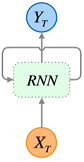
\includegraphics[width=28mm, height=54mm]{rnn.png}
\end{figure}
Architektura LSTM jest w tym momencie najpopularniejszą w zadaniach generowania sekwencji, oraz predykcji szeregów czasowych. Komórka LSTM 
wyposażona jest w trzy bramki: 'wejścia',  'zapomnienia', 'wyjścia'. Bramki te kontrolują które informacje zostaną zapamiętane, zapomniane
oraz przewidziane na podstawie wytrenowanych parametrów. Komórka GRU posiada dwie bramki: 'wejścia' oraz 'zapomnij'. Podobnie do sieci LSTM 
decydują one o tym które informacje mają zostać zachowane, a które zapomniane. CNN to sieć z wyprzedzeniem stosująca operacje splotowe na wejściowych 
wektorach. 

\subsection{Modele statystyczne N-gram}
Model N-gram jest modelem językowym mającym bardzo szerokie zastosowanie we wszystkich dziedzinach związanych z mową oraz pismem. 
N-gramy opierają się na statystykach i służą do przewidywania kolejnego elementu sekwencji.

Modele N-gram szacują prawdopodobieństwo kolejnego słowa na podstawie wcześniej występujących słów za pomocą
prawdopodobieństwa warunkowego. Zatem model przewiduje \begin{math}x_i\end{math} na podstawie danego ciągu 
\begin{math}x_{i-(n-1)},...,x_{i-1}\end{math}. Zapisując wyrażenie przy pomocy prawdopodobieństwa otrzymujemy \\
\centerline{\begin{math}P(x_i|x_{i-(n-1)},...,x_{i-1})\end{math}}

\subsection {Wykorzystany zbiór danych}
\label{sec:dataset-background}
W celach treningowych wykorzystałem zbiór danych zebranych przez grupę SRILAB \cite{dataset}, w celu stworzenia narzędzia 
DeepSyn. Zbiór składa się ze 150 tysięcy plików źródłowych w języku Python, pobranych z serwisu GitHub \cite{github}, po 
usunięciu powtarzających się plików, usunięciu kopii już istniejących repozytoriów oraz zachowaniu tylko programów, z których
można wygenerować poprawne drzewo rozkładu mające co najmniej 30 tysięcy węzłów. Wszystkie projekty wchodzące w skład 
zbioru są wydane na licencjach pozwalających na kopiowanie oraz rozpowszechnianie takich jak MIT, BSD lub Apache. Zbiór jest 
podzielony na 100 tysięcy plików treningowych oraz 50 tysięcy plików walidacyjnych. W swoich eksperymentach użyłem podzbioru 
dostarczonych danych wynoszącego około 1\% oryginalnego zbioru. Decyzja ta wynika z dwóch powodów. Jak wspomniał w swojej 
pracy Hellendoorn i Devanbu\cite{hellendoorn} modele uczenia głębokiego nie skalują dobrze przy dużych danych. Trening na 
pełnym zbiorze byłby niemożliwy ze względu na ograniczenia czasowe. Dla przykładu trening małego modelu LSTM o 512 komórkach 
oraz warstwą zanurzenia (Embedding) na 10 tysiącach plików zabiera około 1.5 godziny dla jednej epoki, na karcie graficznej GeForce RTX 2060. 
Przy założeniu, że czas ten będzie rosnąć proporcjonalnie do rozmiaru danych treningowych, jedna epoka zajmie 
około 15 godzin, a całkowity trening, za który przyjąłem 25 epok, około dwóch tygodni. Drugim jest to, że pracę naukowe, z 
którymi chcę porównać swoje wyniki również używają zbiorów o podobnych rozmiarach. 


    % Umożliwia to również łatwą migrację do nowej wersji szablonu:
\newpage % Rozdziały zaczynamy od nowej strony.
 

\section{Użyte metody}
W tym rozdziale opiszę użyte przez siebie metody prowadzące, od zbioru kodów źródłowych programów, do działającej wtyczki 
przewidującej kolejny token w programie. Omówię również hipotezy zerowe oraz alternatywne dla pytań postawionych w wstępnym rozdziale.\\\\\\ 

\subsection{Badane modele}
Rekurencyjne sieci neuronowe należą do rodziny sieci służących do przetwarzania sekwencji danych o określonej długości. Jak pokazali w swojej publikacji 
Shewalkar, Nyavanandi i Ludwig \cite{lstmvsgru}, sieć LSTM osiąga znacznie lepsze wyniki od podstawowej sieci rekurencyjnej RNN oraz minimalnie lepsze wyniki 
od sieci GRU, kosztem dłuższego czasu treningu. Z tego względu w swoich badaniach skupiam się głównie na warstwie LSTM oraz w mniejszej mierze na warstwie GRU, 
która również wyprzedza podstawową sieć RNN pod względem skuteczności. 

Wszystkie eksperymenty badające wpływ hiperparametrów wymienionych w wstępnym rozdziale \ref{questions} przeprowadzę na sieci LSTM, oraz najlepszą ich kombinację 
zbadam przy wykorzystaniu warstwy GRU w celu porównania ich skuteczności w zadaniu przewidywaniu kodu. Na koniec zbadam również zachowanie wyznaczonego modelu 
dla różnych rozmiarów słownika. 

Jak pokazał w swojej pracy Yoon Kim \cite{kim} połączenie warstwy rekurencyjnej z warstwą zanurzeń poprzez warstwę splotową może mieć pozytywny wpływ na skuteczność 
modelu. Jednak badanie to wykonywał jedynie w zadaniu modelowania języka naturalnego oraz dla modeli opartych na pojedyńczych znakach. Jednym z wykonanych przeze mnie 
eksperymentów będzie zastosowanie tej techniki w moim zadaniu, oraz oceny skuteczności tego podejścia dla modeli opartych na tokenach. \\\\\\

\begin{figure}[!h]
	% Znacznik \caption oprócz podpisu służy również do wygenerowania numeru obrazka;
	\caption{Ogólny badany model. Opcjonalne warstwy zaznaczone linią przerywaną}
	% dlatego zawsze pamiętaj używać najpierw \caption, a potem \label
    \label{fig:architektura}
    % Zamiast width można też użyć height, etc. 
    \centering 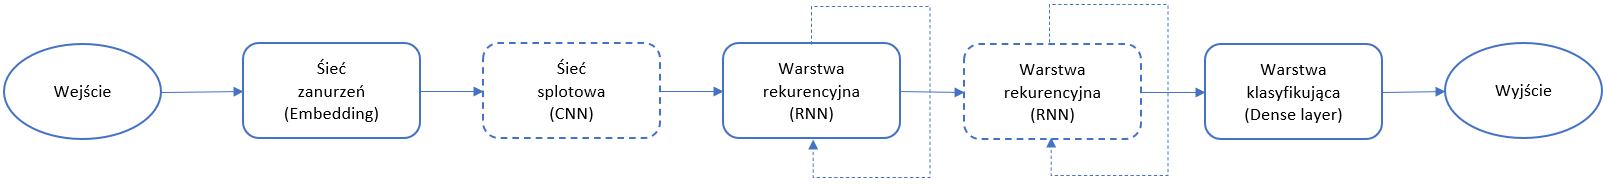
\includegraphics[width=160mm, height=25mm]{architektura.png}
\end{figure}


\begin{table}[ht]
    \centering
    \resizebox{\textwidth}{!}{\begin{tabular}{ccccc}
            \hline
            \multicolumn{1}{|c|}{Długość sekwencji}   & \multicolumn{1}{c|}{Warstwa CNN}          & \multicolumn{1}{c|}{Liczba warstw LSTM} & \multicolumn{1}{c|}{Liczba neuronów w warstwie} & \multicolumn{1}{c|}{Liczba wszystkich parametrów} \\ \hline
            \multicolumn{1}{|c|}{1}                   & \multicolumn{1}{c|}{nie}                  & \multicolumn{1}{c|}{1}                  & \multicolumn{1}{c|}{512}                        & \multicolumn{1}{c|}{todo}                         \\ \hline
            \multicolumn{1}{|c|}{\multirow{5}{*}{5}}  & \multicolumn{1}{c|}{\multirow{4}{*}{nie}} & \multicolumn{1}{c|}{\multirow{3}{*}{1}} & \multicolumn{1}{c|}{128}                        & \multicolumn{1}{c|}{todo}                         \\ \cline{4-5} 
            \multicolumn{1}{|c|}{}                    & \multicolumn{1}{c|}{}                     & \multicolumn{1}{c|}{}                   & \multicolumn{1}{c|}{256}                        & \multicolumn{1}{c|}{todo}                         \\ \cline{4-5} 
            \multicolumn{1}{|c|}{}                    & \multicolumn{1}{c|}{}                     & \multicolumn{1}{c|}{}                   & \multicolumn{1}{c|}{512}                        & \multicolumn{1}{c|}{todo}                         \\ \cline{3-5} 
            \multicolumn{1}{|c|}{}                    & \multicolumn{1}{c|}{}                     & \multicolumn{1}{c|}{2}                  & \multicolumn{1}{c|}{128}                        & \multicolumn{1}{c|}{todo}                         \\ \cline{2-5} 
            \multicolumn{1}{|c|}{}                    & \multicolumn{1}{c|}{tak}                  & \multicolumn{1}{c|}{1}                  & \multicolumn{1}{c|}{128}                        & \multicolumn{1}{c|}{todo}                         \\ \hline
            \multicolumn{1}{|c|}{\multirow{5}{*}{10}} & \multicolumn{1}{c|}{\multirow{4}{*}{nie}} & \multicolumn{1}{c|}{\multirow{2}{*}{1}} & \multicolumn{1}{c|}{128}                        & \multicolumn{1}{c|}{todo}                         \\ \cline{4-5} 
            \multicolumn{1}{|c|}{}                    & \multicolumn{1}{c|}{}                     & \multicolumn{1}{c|}{}                   & \multicolumn{1}{c|}{512}                        & \multicolumn{1}{c|}{todo}                         \\ \cline{3-5} 
            \multicolumn{1}{|c|}{}                    & \multicolumn{1}{c|}{}                     & \multicolumn{1}{c|}{2}                  & \multicolumn{1}{c|}{128}                        & \multicolumn{1}{c|}{todo}                         \\ \cline{3-5} 
            \multicolumn{1}{|c|}{}                    & \multicolumn{1}{c|}{}                     & \multicolumn{1}{c|}{2}                  & \multicolumn{1}{c|}{512}                        & \multicolumn{1}{c|}{todo}                         \\ \cline{2-5} 
            \multicolumn{1}{|c|}{}                    & \multicolumn{1}{c|}{tak}                  & \multicolumn{1}{c|}{1}                  & \multicolumn{1}{c|}{126}                        & \multicolumn{1}{c|}{todo}                         \\ \hline
            \multicolumn{1}{|c|}{\multirow{2}{*}{15}} & \multicolumn{1}{c|}{\multirow{2}{*}{nie}} & \multicolumn{1}{c|}{\multirow{2}{*}{1}} & \multicolumn{1}{c|}{128}                        & \multicolumn{1}{c|}{todo}                         \\ \cline{4-5} 
            \multicolumn{1}{|c|}{}                    & \multicolumn{1}{c|}{}                     & \multicolumn{1}{c|}{}                   & \multicolumn{1}{c|}{512}                        & \multicolumn{1}{c|}{todo}                         \\ \hline
            \end{tabular}}
    \caption{Zestawienie wykonywanych eksperymentów} 
    \label{eksperymenty}
\end{table} 
Zdecydowałem że nie ma potrzeby testowania wszystkich możliwych kombinacji parametrów w tabeli, ponieważ zajęło by to bardzo dużo czasu, oraz już na podstawie prac 
\cite{hellendoorn, pythia} możemy łatwo stwierdzić, że część kombinacji nie osiągnie konkurencyjnych wyników przy pozostałych, na przykład pojedyńcza warstwa LSTM, o 
128 komórkach i długości okna równej \begin{math}1\end{math} jest zdecydowanie za prostym modelem aby przechwycić wszystkie zależności między danymi. 


\subsection{Hipotezy}
Główną hipotezą dla pytania badawczego \ref{questions} jest to, że sieci rekurencyjne sieci neuronowe są w stanie w skuteczny sposób modelować języki programowania. Hipoteza 
ta oparta jest na bardzo dobrych wynikach tego typu sieci w zadaniu modelowania języka naturalnego oraz dużego podobieństwa pomiędzy tymi tymi językami omówionymi wymienionymi 
w sekcji \ref{similarities}. Hipotezę tą popierają również prace Hellendoorn, Devanbu\cite{hellendoorn} oraz Subhasis Das, Chinmayee Shah\cite{contextual_code_completion} uzyskując
obiecujące wyniki przy wykorzystaniu unikalnych metod rozwiązania problemów wiążących się z językami programowania. 
\subsection{Modelowanie tokenów}
Jak pokazuje w swojej publikacji Hao Peng wraz z zespołem \cite{character-level} mimo tego, że modele budujące kolejne słowa poprzez 
przewidywanie pojedyńczego znaku (character-level model) radzą sobie dobrze z modelowaniem języka naturalnego oraz rozwiązują problem rozmiaru słownika, 
działają znacznie gorzej z językami programowania. Wniosek ten również potwierdza w swojej pracy Erik van Scharrenburg \cite{erik} porównując model przewidujący 
znaki z modelem przewidującym tokeny. Z tego powodu w  realizuję tylko modele oparte na tokenach (token-level model). 
\subsubsection{Podpytanie 1}
todo
\subsubsection{Podpytanie 2}
todo
\subsubsection{Podpytanie 3}
todo
\subsubsection{Podpytanie 4}
todo
\subsubsection{Podpytanie 5}
todo

Pierwszym krokiem jest zbudowania słownika tokenów, które mogą pojawić się w kodzie. Buduję go poprzez przetworzenie wszystkich kodów źródłowych obu zbiorów treningowego oraz 
walidacyjnego modułem tokenize \cite{tokenize} wbudowanym w język Python. Moduł ten przyjmuje na wejściu kod źródłowy programu następnie zwraca listę kolejnych tokenów (nazw zmiennych, 
znaków specjalnych, słów kluczowych). Upewnia się on również czy kod jest poprawnie napisany np. czy wszystkie nawiasy lub apostrofy zostały zamknięte. Niepoprawne programy pomijam. 
Znaki nowej lini również traktuję jako token, jednak nie uwzględniam wcięć w kodzie ze względu na to, że większość środowisk programistycznych stawia je 
automatycznie. Na przykład z kodu źródłowego: 
\begin{addmargin}[10mm]{0mm}
    \begin{lstlisting}[
        language=Python,
        numbers=left,
        firstnumber=1,
        caption={Przykładowy program Python},
        aboveskip=10pt
    ]
    for x in range(2, 10): 
        print("hello world")
    \end{lstlisting}
    \end{addmargin}
otrzymamy listę \textbf{ [for, x, in, range, (, 2, 10, ), :, \textbackslash n, print, (, "hello world", )] }.
Następnie sortuje wszystkie wygenerowane tokeny według częstości występowania oraz wybieram top-n tokenów jako słownik i każdemu z nich przypisuję unikalną liczbę naturalną. 
Utworzony w ten sposób słownik nie jest kompletny ponieważ nie obejmuje on wszystkich możliwych nazw występujących w kodzie. Takiego rodzaju tokeny
zostają zastąpione sztucznym tokenem '<UNKNOWN>'. W głównej mierze są to unikalne nazwy zmiennych oraz stringi. Zastępowanie tokenu '<UNKNOWN>' prawdziwym prawdziwym tokenem omawiam w 
rozdziale \ref{oov}

\subsection{Wybór podzbioru danych}
Jak już wspomniałem w sekcji \ref{sec:dataset-background} dotyczącej zbioru danych, trening odbywa sie na podzbiorze wszystkich zgromadzonych danych. W tym celu wybrałem 9 najpopularniejszych 
zewnętrznych bibliotek języka Python stosowanych do zróżnicowanych dziedzin rozwoju oprogramowania. Poniżej zamieszam listę wybranych bibliotek wraz z krótkim opisem:
\begin{itemize}
    \item Django - rozwój aplikacji sieciowych
    \item Numpy - wykonywanie obliczeń matematycznych wysokiego poziomu
    \item Requests - wysyłanie zapytań http 
    \item Flask - rozwój aplikacji sieciowych  
    \item TensorFlow - Głębokie uczenie maszynowe
    \item Keras - Wysokopoziomowe uczenie maszynowe
    \item PyTorch - Głębokie uczenie maszynowe
    \item Pandas - Zarządzanie dużymi zbiorami danych
    \item PyQt - Tworzenie interfejsów użytkownika
\end{itemize} 
Aby upewnić się, że wybrany przeze mnie zbiór danych poprawnie oddaje rzeczywistość porównałem liczbę plików źródłowych zwierających konkretną bibliotekę ze zbioru z odpowiadającą 
liczbą plików źródłowych na platformie GitHub \cite{github}. 
\begin{table}[!h] \centering
    % Znacznik \caption oprócz podpisu służy również do wygenerowania numeru tabeli;
    \caption{Zestawienie zbioru danych z platformą GitHub}
    % dlatego zawsze pamiętaj używać najpierw \caption, a potem \label.
    \label{tab:dataset-compare}
    
    \begin{tabular} {| c | c | r | r |} \hline
        Biblioteka & Liczba plików GitHub & Liczba plików w zbiorze danych & stosunek\\\hline\hline
        Django & 187000000 & 26732 & 0.014\% \\\hline
        Numpy & 55000000 & 9058 & 0.016\% \\ \hline
        Requests & 42000000 & 6339 & 0.015\%\\ \hline
        Pandas & 19000000 & 1328 & 0.007\%\\ \hline
        Flask & 17000000 & 3230 & 0.019\% \\ \hline
        TensorFlow & 10000000 & 96 & 0.001\%\\ \hline
        Keras & 3000000& 72 & 0.002\%\\ \hline
        PyQt & 1000000 & 132 & 0.013\%\\ \hline
        PyTorch & 1000000 & 0 & 0\%\\ \hline
    \end{tabular}
\end{table}

Jak możemy zaobserwować stosunek liczby plików jest dosyć zbliżony dla większości wybranych bibliotek wynosi około 0.015\%, z wyjątkiem 
bibliotek uczenia maszynowego. Może to wynikać z tego, że dane pochodzą z 2018 roku oraz jest to czas, w którym istniały początkowe wersje tych bibliotek oraz dopiero
zaczynały zyskiwać na popularności. Od tego czasu również biblioteka Keras została scalona z biblioteką TensorFlow co znacznie wpłynęło na jej popularność w dzisiejszych czasach. 

Uznaję, że dane w wystarczająco dobrym stopniu oddają częstotliwość zastosowania bibliotek. Końcowy podzbiór stworzyłem poprzez wybranie 1\% plików źródłowych z każdej biblioteki. 
Końcowe zestawienie prezentuje się w następujący sposób:

\begin{table}[!h] \centering
    % Znacznik \caption oprócz podpisu służy również do wygenerowania numeru tabeli;
    \caption{Zestawienie zbioru i podzbioru danych}
    % dlatego zawsze pamiętaj używać najpierw \caption, a potem \label.
    \label{tab:dataset-compare-github}
    
    \begin{tabular} {| c | c | r | r |} \hline
         & Cały zbiór danych & Podzbiór treningowy & Podzbiór walidacyjny \\\hline\hline
        Pliki & 150000 & 9103 & 4504 \\\hline
        Tokeny & 114641650 & 9118453 & 4482600 \\ \hline
    \end{tabular}
\end{table}
Rozmiar wykorzystanego zbioru danych jest podobny do zbioru użytego w publikacjach Vincent J. Hellendoorn i Premkumar Devanbu \cite{hellendoorn} w którym użyto 16 milionów tokenów do treningu, oraz 
5 milionów tokenów w celach walidacji. Na różnicę tą zdecydowałem się ze względu na ograniczenia sprzętowe różniące oba projekty. 


\subsection{Trening}
Zadanie polega na przewidzeniu kolejnego tokenu na podstawie zadanej sekwencji tokenów. Długość sekwencji jest stała oraz wyrażona poprzez wielkość okna będącą jednym z badanych hiperparametrów. 
Dla każdego z tokenów model wyszukuje jego wektor zanurzenia, wykonuje jeden krok w sieci rekurencyjnej po czym stosuje warstwę klasyfikującą 
(Dense layer) w celu wygenerowania logitów wyrażających logistyczne-prawdopodobieństwo kolejnego tokenu. Zatem dla zadanego okna tokenów długości \begin{math}W\end{math}:
\begin{math}[t_1, t_2, ... t_W]\end{math} obliczam wynik dla każdego możliwego wyjścia \begin{math}j, s_j\end{math} jako funkcję z wektorów tokenów \begin{math}v_{t_i}\end{math}
z tokenów z okna.
\\
\centerline{\begin{math}[g_1, g_2, ..., g_W] = RNN([v_{t_1}, v_{t_2}, ..., v_{t_W}])\end{math}}\\
\centerline{\begin{math}s_j=p_{j}^{T}[g]\end{math}} \\\\
Minimalizowana funkcja strat jest entropią krzyżową pomiędzy prawdopodobieństwami \begin{math}softmax\end{math} dla każdego możliwego wyjścia 
a wykonaną predykcją.Funkcja wyrażoną wzorem: \\\\
\centerline{\begin{math}L = log(\frac{e^{s_{t_o}}}{\sum_{j}e^{s_{t_j}}})\end{math}}\\\\
gdzie \begin{math}t_o\end{math} jest zaobserwowanym tokenem wyjściowym a \begin{math}g_i\end{math} wyjściem \begin{math}i^{th}\end{math} komórki
którejś z badanych sieci rekurencyjnych. 

Wagi sieci aktualizowane są po przetworzeniu porcji danych (mini-batch) której rozmiar jest stały. Przy treningach sieci rekurencyjnych rozmiar
ten jest jedną z wartości kluczowych dla dobrej wydajności sieci. W moich eksperymentach wynosi on 128. Jest to kompromis pomiędzy rozsądnym 
czasem treningu oraz jakością wyjściowych sugestii. Jest to również najczęściej wybierana wartość w przytoczonych przeze mnie publikacjach.

Każda testowana sieć trenowana jest przez 25 epoki. Wartość tą wybrałem na podstawie własnych eksperymentów wstępnych, z których wynika, że 
powyżej tej liczby model nie osiągał już lepszych rezultatów. Zbyt długi trening może również doprowadzić to przetrenowania modelu czego 
należy unikać. 

\subsection{Ewaluacja}
Jako, że badane przeze mnie modele tworzone są z myślą użycia ich w postaci wtyczki do środowiska programistycznego nie ma sensu ocenianie ich na podstawie pierwszej, najlepszej predykcji. 
Zamiast tego użyję dwóch następujących metryk: 
\subsubsection{Ewaluacja bez uwzględnienia kolejności}
Jeśli poszukiwane słowo znajduje się w pierwszych \begin{math}n\end{math} najlepszych predykcjach, bez znaczenia na którym miejscu uważam sugestię za poprawną. Metodę tą zastosowano przy ocenianiu systemów
Pythia \cite{pythia} dla której \begin{math}n = 5\end{math} oraz w pracy autorstwa Subhasis Das i Chinmayee Shah \cite{contextual_code_completion} gdzie \begin{math}n = 3\end{math}. Zastosowanie jej pozwoli na porównanie 
wyników z tymi publikacjami. 
\subsubsection{Ewaluacja z uwzględnieniem kolejności}
Jednym z przytoczonym problemów we wstępie \ref{sec:intro} jest to, że wiele wtyczek nie uwzględnia kolejności sugestii oraz proponuje je na przykład posortowane leksykograficznie. Proponowane przeze mnie rozwiązanie 
sortuje predykcje na podstawie prawdopodobieństwa ich wystąpienia. Należy uwzględnić tą kolejność w metryce. Ocena obliczana jest poprzez podzielenie prawdopodobieństwa poprawnego poprawnej predykcji przez 
jego indeks w zbiorze zebranych predykcji. Dla przykładu powiedzmy, że model proponujący 10 sugestii zostaje użyty do wykonania 4 predykcji. Pierwsza wystąpi na 1. miejscu, druga na 3. miejscu, trzecia nie zmieści w w 10 najlepszych, 
a czwarta na 8. miejscu. W takim przypadku ocena modelu będzie wynosić \begin{math}(\frac{1}{1}+ \frac{1}{3}+ 0 +\frac{1}{8})/4 = 0.36\end{math}. W ten sposób wyższe predykcje oceniane są zdecydowanie lepiej.
Przy ocenie użyję 10 najlepszych sugestii.  Metryki tej używa Erik van Scharrenburg \cite{erik} w swojej pracy. Zastosowanie jej pozwoli na porównanie wyników. 

\subsection{Szczegóły implementacji}
\subsubsection{Problem słów poza słownikiem}
\label{oov}
Największym wyzwaniem przy modelowaniu języka programowanie jest rozwiązanie problemu słów poza słownikiem opisanego w podrozdziale \ref{chellenges}. 
Jednym z podejść zastosowanym przez Subhasis Das i Chinmayee Shah jest zastępowanie zastępowanie tokenów nie występujących w słowniku 
specjalnymi tokenami pozycyjnymi. Tego typu tokenowi, który powtarza się więcej niż raz w sekwencji, zostaje przypisany indeks jego wystąpienia 
odpowiadający jego pierwszemu wystąpieniu. W przypadku gdy przewidziany token nie mieści się w słowniku ale pojawił się wcześniej w 
sekwencji zostaje zastąpiony wcześniej podaną nazwą. Rozwiązanie to sprawdza się bardzo dobrze dla zmiennych o tej samej nazwie, znajdujących 
sie blisko siebie, na przykład w pętli \begin{math}for\end{math} języka \begin{math}C++\end{math}: 
\begin{addmargin}[10mm]{0mm}
    \begin{lstlisting}[
        language=C++,
        numbers=left,
        firstnumber=1,
        caption={Przeparsowana pętla for},
        aboveskip=10pt
    ]
    for (int POS_TOKEN_01=0; POS_TOKEN_01<10; POST_TOKEN_01++)
    \end{lstlisting}
    \end{addmargin}
Metoda ta jednak ogranicza się do długości badanej sekwencji, która jest bardzo krótka względem przeciętnej długości kodów programów.


Inną metodą jest zastosowanie warstwy splotowej zamiast warstwy zanurzeń zaproponowaną przez Yoon Kim \cite{kim}. Metoda ta osiąga skuteczność 
na poziomie najlepszych dotychczas znanych modeli jednak zastosowana jest dla modeli języka naturalnego opartego na znakach, przez co 
prawdopodobnie nie sprawdziłaby się przy wybranych przeze mnie założeniach. 

Hellendoorn wraz z Devanbu \cite{hellendoorn} proponują połączenie sieci rekurencyjnych z modelami statystycznymi \begin{math}N-gram\end{math}. Metoda ta pozwala na bardziej 
ogólne predykcje. Pokazują również, że modele \begin{math}N-gram\end{math} radzą sobie lepie z przewidywaniem rzadko występujących unikalnych tokenów od sieci neuronowych, 
oraz kombinacja tych modeli osiąga mniejszą entropię niż każdy z tych modeli osobno. 

Swoje eksperymenty przeprowadzam właśnie z zastosowaniem kombinacji sieci rekurencyjnej z modelami unigram oraz bigram, preferując podpowiedzi wykonane przez bigram. Zastosowanie 
większych modeli \begin{math}N-gram\end{math} nie ma sensu, ponieważ nałożyłoby to dodatkowe koszty obliczeniowe spowalniając wykonywanie predykcji, a generowany przez nie zbiór 
byłby pusty w większości przypadków. 
Stosuje tę metodę poprzez zastąpienie słów nie występujące w słowniku tokenem \begin{math}<UNKNOWN>\end{math} oraz uczę model przewidywać go w odpowiednich miejscach. Następnie jeśli pośród 
zebranych predykcji znajdzie sie token \begin{math}<UNKNOWN>\end{math} zastępuje go zbiorem będącym sumą zbiorów predykcji unigramu oraz bigramu.  
\subsubsection{Rozmiar Słownika}
W eksperymentach z tabeli \ref{eksperymenty} stosuję stałą wartość rozmiaru słownika wynoszącą \begin{math}20000\end{math}. Odpowiada ona usunięciu słów które nie pojawiają sie w 
zbiorze danych więcej niż \begin{math}18\end{math} razy. Odcięte zostają w głównej mierze nazwy zdefiniowanych funkcji, zmiennych oraz stringi.
Wybór ten spowodowany jest tym, że wartość ta ma ogromny wpływ na czas treningu oraz rozmiar modelu zapisanego na dysku. 
Wydłużony czas treningu spowodowany jest koniecznością obliczenia wartości funkcji \begin{math}softmax\end{math} dla każdego ze słów, natomiast dużo większy rozmiar wynika z konieczności 
przeskalowania warstwy wejściowej oraz wyjściowej. Rozmiar ten różni się od rozmiarów wybranych w przytoczonych przeze mnie pracach które wynoszą odpowiednio 74064 \cite{hellendoorn} oraz 
2000 \cite{contextual_code_completion}. W celu odpowiedzi na pytanie czy rozmiar słownika ma znaczenie na badanie modelu przeprowadzę jeden eksperyment polegający na treningu modelu o najlepszej 
skuteczności na rozmiarze słownika 74064 zaproponowanego przez Hellendoorn'a \cite{hellendoorn}. 
Przykłady odciętych tokenów w słowniku rozmiaru 20000:\\ \begin{math}accept\_inplace, IVGMM, book\_names, allvars, parent\_cards, 'references'\end{math}
\subsubsection{Wektory zanurzenia}
Wektory zanurzeń odpowiedzialne są za przypisaniu każdemu ze słów wektora, którym możemy wyrazić prawdopodobieństwo tokenu jako rezultat wielowarstwowej sieci neuronowej na wektorach 
o ograniczonej liczbie tokenów sąsiednich. T. Milolv \cite{word2vec} pokazuje, że taki model wykrywa relacje między parami słów na przykład słowo 'król' ma sie do 'królowa' tak samo 
jak 'mężczyzna' do 'kobieta'. Warstwa zanurzeń jets pierwszą warstwą w modelu.
Wymiary wektorów zanurzeń są stałe dla każdego z wykonywanych eksperymentów oraz wynoszą one \begin{math}32\end{math}. Zdecydowałem się na mniejszy wymiar wektorów niż przedstawiony 
w pracy \cite{hellendoorn}, która wynosiła 128 z powodu, że używam mniejszego słownika przez co znajduję się w nim dużo mniej zależności, które można wyrazić mniejszym wymiarem. 
\subsubsection{Optymalizator}
W treningu używam optymalizatora \begin{math}Adam\end{math} o domyślnych parametrach dla każdego z modeli.
Wybór ten wynika z tego, że zależy mi na badaniu różnic wynikających z badanej architektury oraz odpowiednie strojenie optymalizatora typu SGD
było by bardzo czasochłonne oraz bardzo komplikowałoby porównywanie ze sobą testowanych modeli. Jest to również optymalizator używany w pracach 
z którymi porównam uzyskane przeze mnie wyniki.  

 % wystarczy podmienić swoje pliki main.tex i eiti-thesis.cls
                            % na nowe wersje, a cały tekst pracy pozostaje nienaruszony.
\newpage % Rozdziały zaczynamy od nowej strony.
 

\section{Analiza przeprowadzonych eksperymentów}

\subsection{Zbadane architektury}
\subsection{Wyróżniona architektura}
\subsection{Różne rozmiary słownika}
\subsection{Zastosowanie warstwy GRU}
\subsection{Najlepsza znaleziona architektura}

\newpage % Rozdziały zaczynamy od nowej strony.
 

\section{Implementacja wtyczki}
\subsection{Architektura klient-serwer}
\subsection{Obsługa}
  


\newpage % Rozdziały zaczynamy od nowej strony.
 

\section{Podsumowanie}





%--------------------------------------------
% Literatura
%--------------------------------------------
\cleardoublepage % Zaczynamy od nieparzystej strony
\printbibliography

%--------------------------------------------
% Spisy (opcjonalne)
%--------------------------------------------
\newpage
\pagestyle{plain}

% Wykaz symboli i skrótów.
% Pamiętaj, żeby posortować symbole alfabetycznie
% we własnym zakresie. Ponieważ mało kto używa takiego wykazu,
% uznałem, że robienie automatycznie sortowanej listy
% na poziomie LaTeXa to za duży overkill.
% Makro \acronymlist generuje właściwy tytuł sekcji,
% w zależności od języka.
% Makro \acronym dodaje skrót/symbol do listy,
% zapewniając podstawowe formatowanie.
% //AB
\vspace{0.8cm}
\acronymlist
\acronym{EiTI}{Wydział Elektroniki i Technik Informacyjnych}
\acronym{PW}{Politechnika Warszawska}

\listoffigurestoc     % Spis rysunków.
\vspace{1cm}          % vertical space
\listoftablestoc      % Spis tabel.
\vspace{1cm}          % vertical space
\listofappendicestoc  % Spis załączników

% Załączniki
% \newpage
% \appendix{Nazwa załącznika 1}
% \lipsum[1-8]

% \newpage
% \appendix{Nazwa załącznika 2}
% \lipsum[1-4]

% Używając powyższych spisów jako szablonu,
% możesz tu dodać swój własny wykaz bądź listę,
% np. spis algorytmów.

\end{document} % Dobranoc.
